\section{Semi-global alignment and mapping}

\begin{floatingfigure}[l]{0.5\textwidth}
    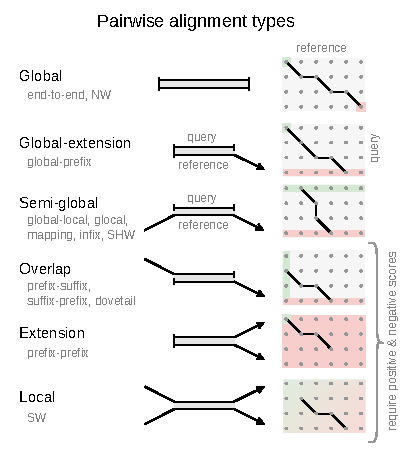
\includegraphics[width=0.5\textwidth]{alignment-types}
	\caption[Alignment types]{Alignment types.}
    \label{fig:alignment-types}
\end{floatingfigure}

% paper-trie; seed-and-extend approach to semi-global alignment
\para{Seed-and-Extend}
Since optimal alignment is often intractable, many aligners use heuristics, most
commonly the \emph{seed-and-extend}
paradigm~\cite{altschul_basic_1990,langmead_fast_2012,li_fast_2009}. In this
approach, alignment initiation sites (\emph{seeds}) are determined, which are
then \emph{extended} to form the \emph{alignments} of the query sequence. The
fundamental issue with this approach, however, is that the seeding and extension
phases are mostly decoupled during alignment. Thus, an algorithm with a provably
optimal extension phase may not result in optimal alignments due to the
selection of a suboptimal seed in the first phase. In cases of high sequence
variability, the seeding phase may even fail to find an appropriate seed from
which to extend.

%%%%%%%%%%%%%%%%%%%%%%%%%%%%%%%%%
\subsection{Related work}

% Brownie aligner
BrownieAligner, another recent work developed for local alignment of sequences
to {\itshape de Bruijn} graph representations of genomic variation, features an
optimal extension phase using a branch-and-bound-based early cutoff, while
employing a heuristic maximal-exact-match approach for
seeding~\cite{heydari_browniealigner_2018}.